\Chapter{PREMIER PASSAGE EN DIFFUSION AVEC SAUTS}\label{sec:FPT_Jump}
Ce chapitre se concentre sur la variante discontinue du \acs{CIR}. Le processus est donc défini comme suit:
\begin{equation}\label{jump_cir_sde}
    X(t)=X(0)+\int_0^t a(b-X(s))ds+\int_0^t\sigma\sqrt{X(s)}dW(s)+J(t)
\end{equation}
avec
\begin{itemize}
    \item $X(0)=x$;
    \item $W(t)$ un \acs{MBS};
    \item $J(t)$ un processus de sauts pur comme défini en (\ref{jump_def}).
\end{itemize}

\section{Fonction Temps Moyen \textemdash~Sauts Uniformes Descendants}\label{subsection_mean_jumps}
\subsection{Résolution du problème}
Dans cette section, la variante du \ac{CIR} avec sauts considérée est celle avec des sauts négatifs modélisés par des variables uniformément distribuées sur $[-x,0]$. La mesure d'intensité des sauts est donc:
\[
\gamma(dy)=\lambda\frac{1}{x}\mathds{1}_{y\in[-x,0]}dy
\]

\paragraph{Dérivation de l'équation à résoudre}\phantom{}\\
En reprenant ce qui avait été fait en (\ref{section_fgm_eq}) pour dériver l'\acs{EDO} régissant la \acl{FGM} de $\tau(x)$, il est possible d'écrire:
\[
\frac{1}{2}\sigma^2 xM''(x;\alpha)+a(b-x)M'(x;\alpha)+\lambda\left\{\frac{1}{x}\int_{-x}^0M(x+y;\alpha)dy-M(x;\alpha)\right\}-\alpha M(x;\alpha)=0
\]
avec $M(0;\alpha)=M(c;\alpha)=1$.

Ensuite, en procédant comme dans (\ref{section_mean_eq}), il découle l'équation du temps moyen de sortie de l'intervalle pour le processus avec sauts:
\begin{equation}\label{mean_ide}
    \frac{1}{2}\sigma^2 xm''(x)+a(b-x)m'(x)+\lambda\left\{\frac{1}{x}\int_{-x}^0m(x+y)dy-m(x)\right\}=-1
\end{equation}
avec $m(0)=m(c)=0$.

Soit le changement de variable suivant:
\begin{equation}\label{variable_change_mean}
    \int_{-x}^0m(x+y)dy=\int_0^x m(z)dz
\end{equation}
La formule de Leibniz permet d'écrire:
\[
\frac{d}{dx}\left(\int_0^x m(z)dz\right)=m(x)
\]
Donc, en dérivant les deux côtés de l'équation (\ref{mean_ide}) et en éliminant le retour à la moyenne ($a=0$), il découle une \acs{EDO} d'ordre 3:
\begin{equation}\label{mean_3rd_order}
    \frac{1}{2}\sigma^2xm'''(x)+\sigma^2m''(x)-\lambda m'(x)=-\frac{1}{x}
\end{equation}

\paragraph{Résolution}\phantom{}\\
Soit les valeurs suivantes des paramètres: $\sigma=\sqrt{2}$, $\lambda=1$ et $c=1$. \textit{Maple} donne comme solution:
\begin{equation}\label{sol_mean_with_jumps}
    m(x)=C_1I_0(2\sqrt{x})+C_2K_0(2\sqrt{x})+2\ln(2\sqrt{x})+C_3
\end{equation}
avec $C_1$, $C_2$, $C_3$ des constantes à déterminer et $I_0(\cdot)$, $K_0(\cdot)$ les fonctions de Bessel modifiées de première et seconde espèce respectivement (voir annexe~\ref{special_functions}).

Les constantes $C_1$, $C_2$ et $C_3$ sont déterminées en imposant les conditions aux limites $m(0)=m(1)=0$ ainsi qu'une condition supplémentaire $m(0.5)=r$. Ensuite, la valeur de $r$ permettant de satisfaire l'équation originale (\ref{mean_ide}) est trouvée: $r\simeq0.3281$.

\paragraph{Étude du cas sans sauts}\phantom{}\\
Afin de comparer l'effet de la présence des sauts, il est intéressant de résoudre le même problème en retirant ces derniers. Soit $m_0(x)$ le temps moyen de sortie du processus sans sauts. En considérant les mêmes valeurs des paramètres, l'équation à résoudre devient:
\begin{equation}\label{mean_3rd_order_without_jumps}
    xm_0''(x)=-1
\end{equation}
La solution qui satisfait $m_0(0)=m_0(1)=0$ est:
\begin{equation}\label{sol_mean_with_0_jumps}
    m_0(x)=-x\ln(x)
\end{equation}

\subsection{Validation de l'expression obtenue}
Les fonctions \( m(x) \) (avec sauts) et \( m_0(x) \) (sans sauts), données respectivement par (\ref{sol_mean_with_jumps}) et (\ref{sol_mean_with_0_jumps}), sont tracées.
\paragraph{Visualisation}\phantom{}
\begin{figure}[htb]
    \centering
    \begin{subfigure}{0.45\linewidth}
        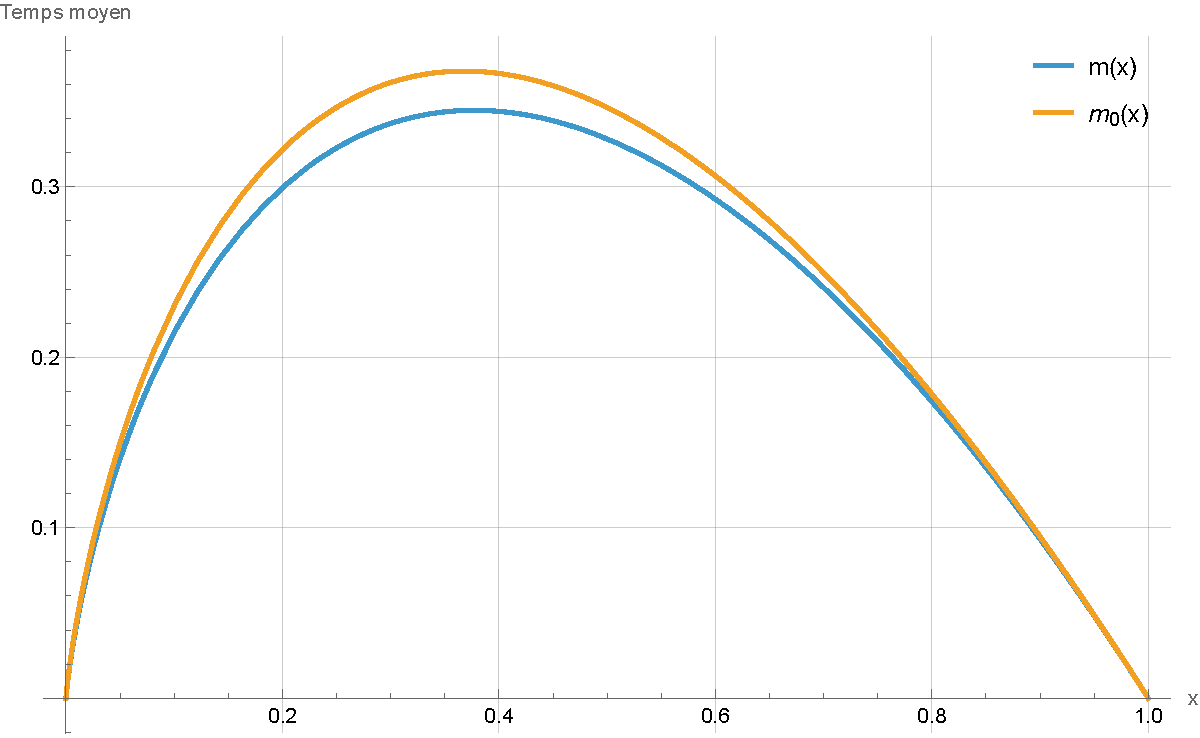
\includegraphics[width=\linewidth]{img/validation/Jumps/mean_jumps.pdf}
        \caption{Fréquence des sauts $\lambda=1$}
    \end{subfigure}
    \hfill
    \begin{subfigure}{0.45\linewidth}
        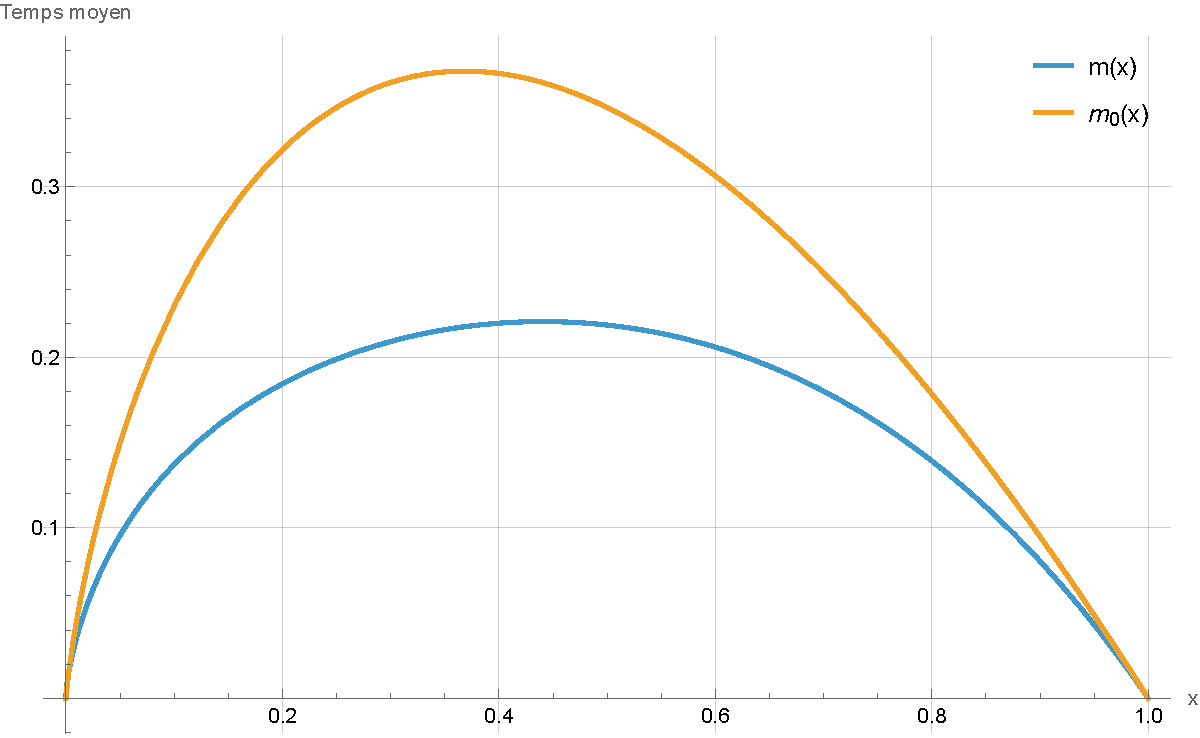
\includegraphics[width=\linewidth]{img/validation/Jumps/mean_big_jumps.pdf}
        \caption{Fréquence des sauts $\lambda=10$}
    \end{subfigure}
    \caption{Visualisation des temps moyens de sortie $m(x)$ et $m_0(x)$}\label{fig:JumpsMeanVisualisation}
\end{figure}
\FloatBarrier\paragraph{Analyse}\phantom{}\\
Il convient de souligner les observations suivantes:
\begin{itemize}
    \item Les conditions aux limites \( m(0) = m(c) = m_0(0) = m_0(c) = 0 \) sont bien vérifiées;
    \item Le temps moyen de sortie en présence de sauts ($m(x)$ en bleu) est inférieur à celui observé sans sauts ($m_0(x)$ en orange), ce qui illustre l'accélération du processus induite par ces derniers;
    \item Une augmentation de la fréquence des sauts $\lambda$ induit une diminution du temps moyen de sortie. Ce comportement est attendu comme les sauts augmente la probabilité que le \acs{CIR} quitte l'intervalle rapidement.
\end{itemize}
La fonction obtenue pour le temps moyen de sortie avec sauts est donc validée.

\section{Fonction Probabilité de Sortie en Zéro \textemdash~Sauts Uniformes Descendants}\label{subsection_probability_jumps}
\subsection{Résolution du problème}
Dans cette section, la variante du \ac{CIR} avec sauts considérée est identique à la précédente (sauts négatifs modélisés par des variables uniformément distribuées sur $[-x,0]$).

\paragraph{Dérivation de l'équation à résoudre}\phantom{}\\
Il est possible de montrer (voir~\cite{lefebvre2007}) que la fonction probabilité de sortie en zéro satisfait l'\acs{EDO}:
\begin{equation}\label{probability_ide}
    \frac{1}{2}\sigma^2xp''(x)+a(b-x)p'(x)+\lambda\left\{\frac{1}{x}\int_{-x}^0p(x+y)dy-p(x)\right\}=0
\end{equation}
sous les conditions $p(0)=1$ et $p(c)=0$.

Ensuite, en effectuant le même changement de variable que pour la fonction temps moyen (\ref{variable_change_mean}), en dérivant les deux membres de l'équation et en éliminant le retour à la moyenne ($a=0$), il découle:
\begin{equation}\label{probability_3rd_order}
    \frac{1}{2}\sigma^2xp'''(x)+\sigma^2p''(x)-\lambda p'(x)=0
\end{equation}
\paragraph{Résolution}\phantom{}\\
En reprenant les mêmes valeurs des paramètres ($\sigma=\sqrt{2}$, $\lambda=1$ et $c=1$) et en imposant les conditions $p(0)=1$, $p(1)=0$ et $p(0.5)=r$, \textit{Maple} donne la solution suivante:
\begin{equation}\label{sol_probability_with_jumps}
    p(x)=\frac{I_0(2)-I_0(2\sqrt{x})}{I_0(2)-1}
\end{equation}
avec $I_0(\cdot)$ la fonction de Bessel modifiée de première espèce (voir annexe~\ref{special_functions}) et $r\simeq0.5567$.
\paragraph{Étude du cas sans sauts}\phantom{}\\
Dans la même logique, le même problème en absence des sauts est résolu pour $p_0(x)=\mathds{P}[X(\tau(x))=0]$. L'équation (\ref{probability_3rd_order}) devient:
\[
xp_0''(x)=0
\]
La solution qui satisfait $p(0)=1$ et $p(1)=0$ est:
\begin{equation}\label{sol_probability}
    p_0(x)=1-x
\end{equation}
\subsection{Validation de l'expression obtenue}
Les fonctions \( p(x) \) (avec sauts) et \( p_0(x) \) (sans sauts), correspondant respectivement aux expressions (\ref{sol_probability_with_jumps}) et (\ref{sol_probability}), sont représentées graphiquement.
\paragraph{Visualisation}\phantom{}
\begin{figure}[htb]
    \centering
    \begin{subfigure}{0.45\linewidth}
        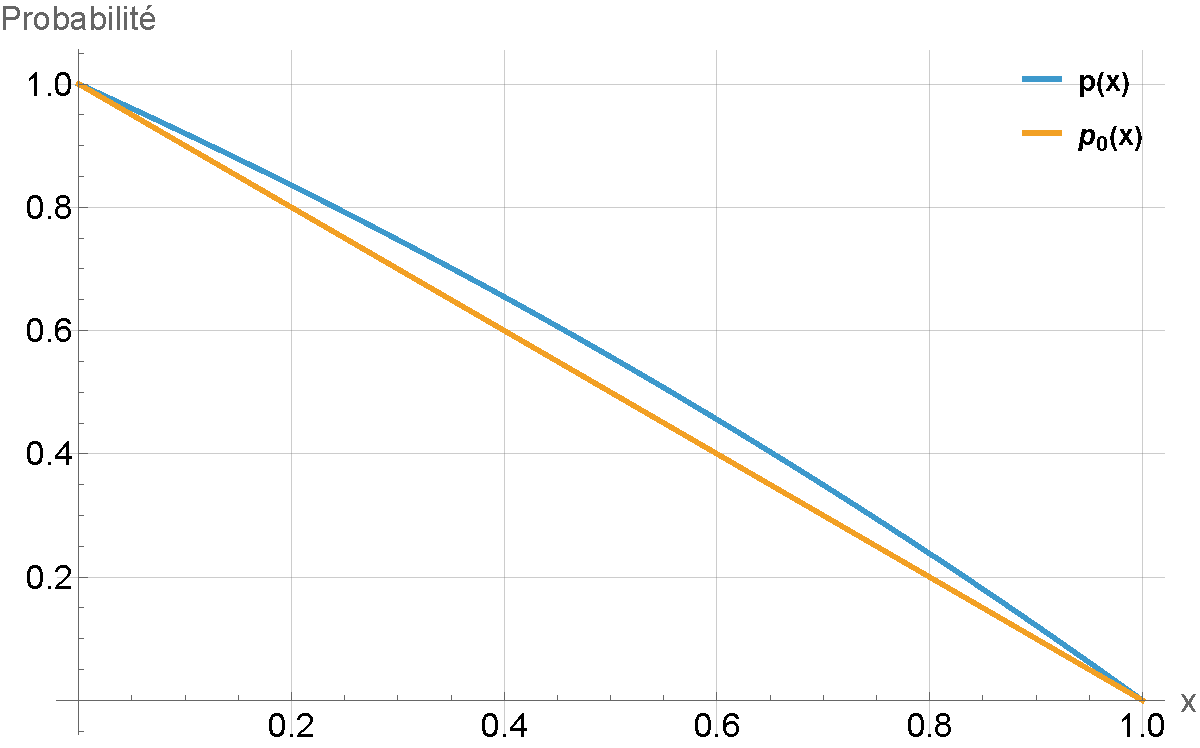
\includegraphics[width=\linewidth]{img/validation/Jumps/probability_jumps.pdf}
        \caption{Fréquence des sauts $\lambda=1$}
    \end{subfigure}
    \hfill
    \begin{subfigure}{0.45\linewidth}
        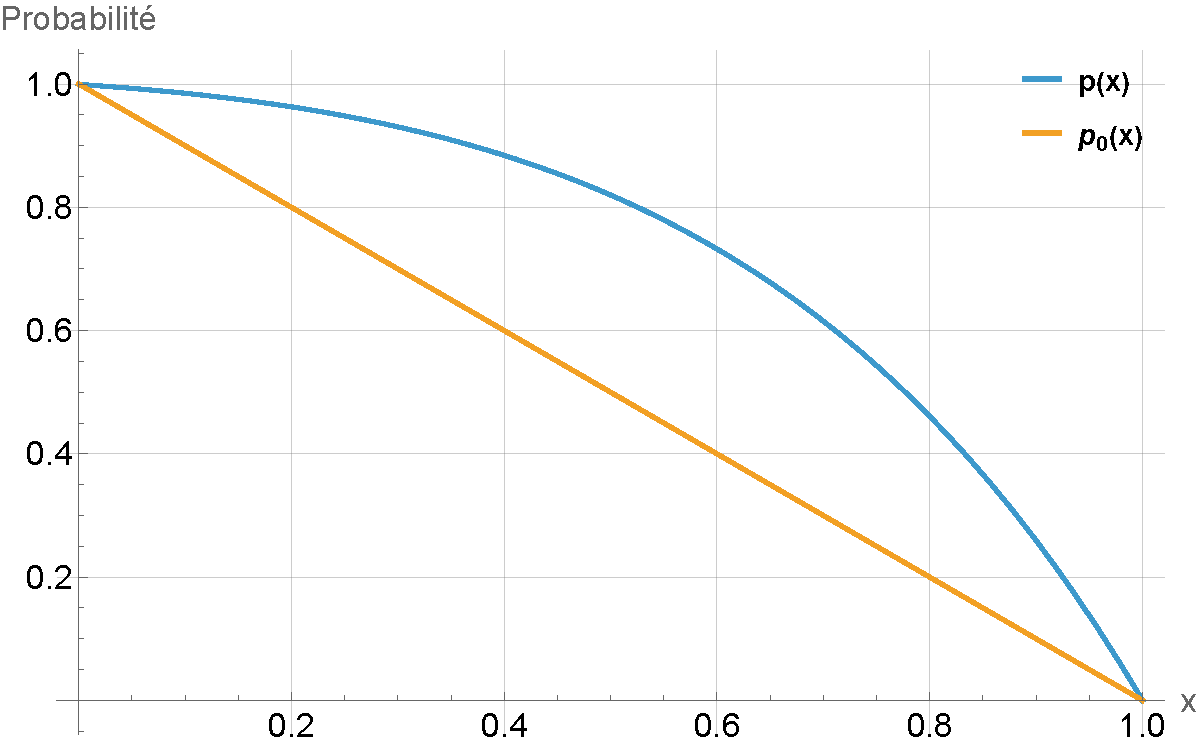
\includegraphics[width=\linewidth]{img/validation/Jumps/probability_big_jumps.pdf}
        \caption{Fréquence des sauts $\lambda=10$}
    \end{subfigure}
    \caption{Visualisation des probabilités de sortir en zéro $p(x)$ et $p_0(x)$}\label{fig:JumpsProbabilityVisualisation}
\end{figure}
\FloatBarrier\paragraph{Analyse}\mbox{}\\
Les observations suivantes peuvent être formulées:
\begin{itemize}
    \item Les conditions aux limites sont correctement satisfaites, à savoir \( p(0) = p_0(0) = 1 \) et \( p(c) = p_0(c) = 0 \);
    \item Les sauts étant négatifs, ils favorisent une sortie par la borne inférieure. La probabilité de franchissement par zéro est donc plus élevée dans le cas avec sauts ($p(x)$ en bleu);
    \item Une augmentation de la fréquence des sauts $\lambda$ entraîne une augmentation considérable de la probabilité de sortir par zéro. En effet, la multiplication des sauts tend à entraîner le processus vers la borne inférieure.
\end{itemize}
Ces résultats permettent donc de valider l'expression obtenue pour la probabilité de sortie en zéro.

\section{Fonction Dépassement Moyen \textemdash~Sauts Exponentiels Ascendants}
\subsection{Formulation générale du problème}
\paragraph{Théorème} 
\textit{Soit \(\{X(t),\,t \geq 0\}\) un processus de diffusion à sauts vérifiant les conditions d'unicité des trajectoires (\ref{trajecotry_uniqueness}), et défini par:}
\[
X(t) = X(0) + \int_0^t \mu(X(s))\,ds + \int_0^t \sigma(X(s))\,dW(s) + J(t)
\]
\textit{où \(J(t)\) est un processus de sauts pur associé à une mesure d'intensité \(\gamma(dy)\).}  

\textit{Alors, la fonction \(D(x)\) (\ref{overshoot}), représentant le dépassement moyen au-dessus de la frontière \(c\) au temps du premier passage \(\tau(x)\) (\ref{fpt_definition}), satisfait l'équation suivante:}
\begin{equation}\label{general_overshoot_ide}
    \mathcal{L}D(x) = -\int_{c - x}^{+\infty} (x + y - c)\,\gamma(dy)
\end{equation}
\textit{avec \(D(0) = D(c) = 0\) et \(\mathcal{L}\) le générateur infinitésimal du processus (voir~\ref{infinitesimal_generator}).}

\paragraph{Démonstration}
Soit $f(x)={(x-c)}_+$ la fonction mesurant un dépassement. En appliquant la formule de Dynkin (voir~\cite{dynkin1965}), il est possible d'écrire:
\begin{equation}\label{initial_dynkin}
    \mathds{E}[f(X(\tau(x)))]=f(x)+\mathds{E}\left[\int_0^{\tau(x)}\mathcal{L}f(X(s))ds\right]
\end{equation}
Pour $x\in(0,c)$:
\begin{itemize}
    \item $f(x)={(x-c)}_+=0$
    \item $f'(x)=\mathds{1}_{x\geq c}=0\implies f''(x)=0$
\end{itemize}
Le générateur infinitésimal (\ref{infinitesimal_generator}) devient:
\[
\begin{aligned}
    \mathcal{L}f(x) &= \frac{1}{2}\sigma^2(x)f''(x)+\mu(x)f'(x)+\int_{\mathds{R}}[f(x+y)-f(x)]\gamma(dy)\\
    &=\int_{\mathds{R}}(x+y-c)_+\,\gamma(dy) \\
    &=\int_{c-x}^{+\infty}(x+y-c)\gamma(dy)
\end{aligned}
\]
Le dépassement moyen est donc:
\[
D(x):=\mathds{E}\left[{(X(\tau(x))-c)}_+\right]=\mathds{E}[f(X(\tau(x)))]=\mathds{E}\left[\int_0^{\tau(x)}\left(\int_{c-x}^{+\infty}(X(s)+y-c)\gamma(dy)\right)ds\right]
\]
Alors, Abundo~\cite{abundo2013} a montré que $D(x)$ satisfait:
\[
\mathcal{L}D(x) = -\int_{c - x}^{+\infty} (x + y - c)\,\gamma(dy)
\]
avec $D(0)=D(c)=0$.\hfill$\square$

\subsection{Sauts exponentiels ascendants}
\paragraph{Lemme} 
\textit{Sous les mêmes hypothèses que précédemment, et en supposant que les sauts suivent une loi exponentielle de paramètre \(\nu > 0\) avec une intensité \(\lambda > 0\), la fonction \(D(x)\) (\ref{overshoot}) satisfait l'équation différentielle homogène d'ordre trois suivante:}
\begin{equation}\label{eq:general_ode_D}
    \begin{aligned}
        \sigma(x)^2 D'''(x)+D''(x) \left[2 \mu(x)+\sigma(x)(2\sigma'(x)-\nu  \sigma(x))\right]\\-2D'(x)[\lambda-\mu'(x)+\nu\mu(x)]=0
    \end{aligned}
\end{equation}
\textit{avec \(D(0) = D(c) = 0\).}

\paragraph{Démonstration}
Si la mesure d'intensité s'écrit:
\[
\gamma(dy):=\lambda\nu e^{-\nu y}\mathds{1}_{y\geq0}dy
\]
Alors:
\[
\int_{c-x}^{+\infty}(x+y-c)\gamma(dy)=\frac{\lambda}{\nu e^{\nu c}}e^{\nu x}
\]
L'équation (\ref{general_overshoot_ide}) devient:
\begin{equation}\label{initial_overshoot_ide}
    \frac{1}{2}\sigma^2(x)D''(x)+\mu(x)D'(x)+\lambda\int_0^\infty[D(x+y)-D(x)]\nu e^{-\nu y}dy=-\frac{\lambda}{\nu e^{\nu c}}e^{\nu x}
\end{equation}
D'abord, l'intégrale peut être simplifiée: 
\begin{equation}\label{simplified_overshoot_ide}
    \frac{1}{2}\sigma^2(x)D''(x)+\mu(x)D'(x)+\lambda\int_0^\infty D(x+y)\nu e^{-\nu y}dy-\lambda D(x)=-\frac{\lambda}{\nu e^{\nu c}}e^{\nu x}
\end{equation}
Le changement de variable $z=x+y$ donne:
\[
\begin{aligned}
    \int_0^\infty D(x+y)\nu e^{-\nu y}dy&=\int_x^\infty D(z)\nu e^{-\nu(z-x)}dz\\
    &=\nu e^{\nu x}\int_x^\infty D(z)e^{-\nu z}dz
\end{aligned}
\]
Soit:
\[
\Phi(x):=\int_x^\infty D(z)e^{-\nu z}dz
\]
L'équation (\ref{simplified_overshoot_ide}) devient:
\begin{equation}\label{ODE_Phi_D}
    \frac{1}{2}\sigma^2(x)D''(x)+\mu(x)D'(x)+\lambda\nu e^{\nu x}\Phi(x)-\lambda D(x)=-\frac{\lambda}{\nu e^{\nu c}}e^{\nu x}
\end{equation}
D'une part, la dérivée de $\Phi(x)$ est (règle de Leibniz):
\begin{equation}\label{Leibniz_rule}
    \Phi'(x)=-D(x)e^{-\nu x}\implies D(x)=-e^{\nu x }\Phi'(x)
\end{equation}
D'autre part, les dérivées de $D(x)$ s'écrivent: 
\begin{equation}\label{eq:d_derivees}
    \begin{aligned}
        D'(x) &= -\nu e^{\nu x}\Phi'(x)-e^{\nu x}\Phi''(x) \\
        D''(x)&= -\nu^2e^{\nu x}\Phi'(x)-2\nu e^{\nu x}\Phi''(x)-e^{\nu x}\Phi'''(x)
    \end{aligned}
\end{equation}
En injectant (\ref{eq:d_derivees}) dans (\ref{ODE_Phi_D}) et en éliminant les termes $-e^{\nu x}$, il découle l'\acs{EDO} d'ordre 3 suivante: 
\begin{equation}\label{general_ode_Phi}
    \begin{aligned}
        \frac{1}{2}\sigma^2(x)\Phi'''(x)+\Phi''(x)\left[\nu\sigma^2(x)+\mu(x)\right]\\+\Phi'(x)\left[\frac{1}{2}\nu^2\sigma^2(x)+\nu\mu(x)-\lambda\right]-\lambda\nu\Phi(x)=\frac{\lambda}{\nu e^{\nu c}}
    \end{aligned}
\end{equation}
Comme $D(x)$ ne dépend que de $\Phi'(x)$ (\ref{Leibniz_rule}), il est intéressant de dériver l'équation ci-dessus (\ref{general_ode_Phi}) en posant $\phi(x)=\Phi'(x)$ pour obtenir l'\acs{EDO} homogène suivante:
\begin{equation}\label{general_ode_phi}
    \begin{aligned}
        \sigma(x)^2 \phi'''(x)+2 \phi''(x) \left[\mu(x)+\sigma(x) \left(\sigma'(x)+\nu  \sigma(x)\right)\right]\\+\phi'(x) \left[-2 \lambda +2 \mu'(x)+2 \nu\mu(x)+\nu  \sigma(x) \left(4 \sigma'(x)+\nu  \sigma(x)\right)\right]\\+2 \nu  \phi(x) \left[-\lambda +\mu'(x)+\nu  \sigma(x) \sigma'(x)\right]=0
    \end{aligned}
\end{equation}
avec $D(x)=-e^{\nu x}\Phi'(x)=-e^{\nu x}\phi(x)$ et $\phi(0)=\phi(c)=0$.

Ensuite, il est possible de montrer que $\phi_1(x)=e^{-\nu x}$ est une solution particulière de (\ref{general_ode_phi}). La solution générale s'écrit donc: 
\[
\begin{aligned}
    D(x)&=-e^{\nu x}\phi(x)\\
    &=-e^{\nu x}\phi_1(x)u(x)\\
    &=-e^{\nu x}e^{-\nu x}u(x)\\
    &=-u(x)
\end{aligned}
\]
avec $u(x)$ une fonction à déterminer. En effectuant un changement de variable avec la solution particulière et en échangeant $u$ par $-D$, l'\acs{EDO} homogène d'ordre 3 suivante est obtenue: 
\[
    \begin{aligned}
        \sigma(x)^2 D'''(x)+D''(x) \left[2 \mu(x)+\sigma(x)(2\sigma'(x)-\nu  \sigma(x))\right]\\-2D'(x)[\lambda-\mu'(x)+\nu\mu(x)]=0
    \end{aligned}
\]
avec $D(0)=D(c)=0$.\hfill$\square$\\

Cette équation permet donc de résoudre le problème pour tout processus \(\{X(t),\,t\geq0\}\). Dans la suite, le \acs{CIR} avec sauts exponentiels est considéré.
\subsection{Application au CIR}
En reprenant les termes de dérive et de diffusion du \acs{CIR} (\ref{cir_eq}), l'équation (\ref{eq:general_ode_D}) devient:
\[
\sigma ^2 x D'''(x)+D''(x) \left[2 a (b-x)+\sigma ^2-\nu  \sigma ^2x\right]-2 D'(x) [a \nu  (b-x)+a+\lambda ]=0
\]
Cependant, une expression explicite pour $D(x)$, si elle existe, est très difficile à obtenir. Cela rend donc la résolution du problème général assez compliqué. 
\paragraph{Résolution pour $a=0$}\phantom{}\\
En considérant le cas du \acs{CIR} à sauts sans retour à la moyenne ($a=0$) et en posant \(\sigma=c=\lambda=\nu=1\), \textit{Maple}  donne l'expression suivante:
\begin{equation}\label{overshoot_exact_sol}
    D(x)=2xe^{x}\left[E_1(x)-E_1(1)\right]
\end{equation}
avec $E_n(x)$ la fonction intégrale exponentielle généralisée (voir annexe~\ref{special_functions}).
\paragraph{Détermination des constantes}\phantom{}\\
Les conditions aux limites $D(0)=D(c)=0$ permettent de déterminer les deux constantes $C_1$ et $C_2$. Étant donné la longueur des expressions obtenues, celles-ci ne seront pas détaillées dans le présent document.

\subsection{Validation de l'expression obtenue}
\paragraph{Visualisation}\phantom{}\\
Afin de valider le résultat, l'expression obtenue pour $D(x)$ (\ref{overshoot_exact_sol}) est tracée.
\begin{figure}[htb]
    \centering
    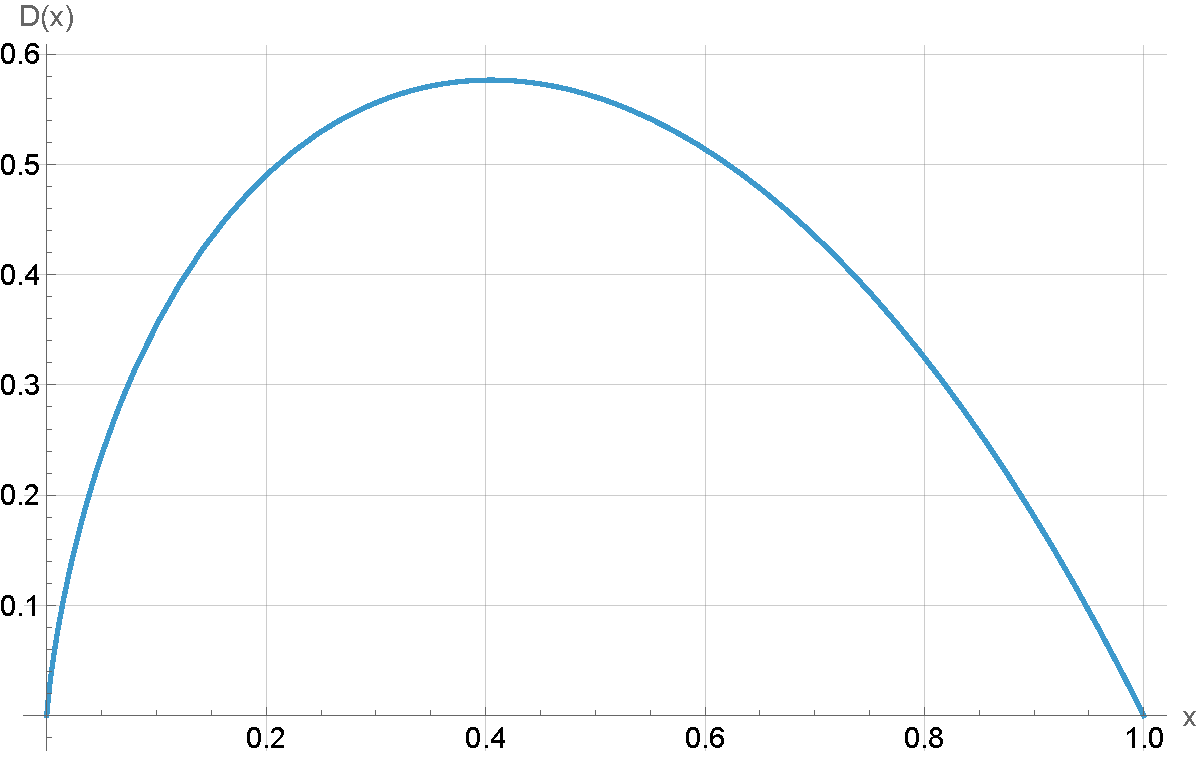
\includegraphics[width=0.5\linewidth]{img/validation/Ovs/exact.pdf}
    \caption{Visualisation de la fonction Dépassement Moyen $D(x)$}\label{fig:OvershootExactSol}
\end{figure}
\FloatBarrier\paragraph{Analyse}\phantom{}\\
Les différents points suivants sont relevés:
\begin{itemize}
    \item Les conditions aux limites $D(0)=D(c)=0$ sont respectées;
    \item La fonction représente un \textit{dépassement moyen}, elle doit donc être positive pour toute valeur $x$ dans $[0,c]$;
    \item Une augmentation de la fréquence des sauts $\lambda$ induit une augmentation du dépassement moyen. En effet, il devient plus probable que le processus effectue un saut juste avant d'atteindre la frontière, ce qui augmente les chances de la franchir avec un certain excès;
\end{itemize}
La fonction Dépassement Moyen $D(x)$ est donc validée.

